\documentclass[conference]{IEEEtran}
\IEEEoverridecommandlockouts
\usepackage{cite}
\usepackage{amsmath,amssymb,amsfonts}
\usepackage{graphicx}
\usepackage{textcomp}
\usepackage{xcolor}
\usepackage{booktabs}
\usepackage{url}
\usepackage{listings}
\lstset{basicstyle=\small\ttfamily, breaklines=true, breakatwhitespace=true,
        frame=none, xleftmargin=0pt}
\def\BibTeX{{\rm B\kern-.05em{\sc i\kern-.025em b}\kern-.08em
    T\kern-.1667em\lower.7ex\hbox{E}\kern-.125emX}}
\graphicspath{{img/}}
\begin{document}

\title{A gm/Id Methodology Design Tool for Analog CMOS Circuit Synthesis:\\
Application to the Folded-Cascode Class-AB Amplifier}

\author{\IEEEauthorblockN{Phil Alcorn}
\IEEEauthorblockA{\textit{Department of Electrical Engineering} \\
\textit{Tarleton State University}\\
Stephenville, TX \\
palcorn2000@gmail.com}
}

\maketitle

\begin{abstract}
This paper presents a Python-based simulation pipeline that automates the
gm/Id transistor sizing methodology for CMOS analog circuits.  The tool
characterizes NMOS and PMOS transistors across channel length, gate-to-source
voltage, drain-to-source voltage, and bulk-to-source voltage using LTspice
operating-point sweeps, stores the results in a four-dimensional look-up
table (LUT), and provides a query interface for transistor sizing.  The
design flow is demonstrated by applying the extracted LUTs to the sizing of
a folded-cascode class-AB operational amplifier, walking through each
transistor group from specification to final width.
\end{abstract}

\begin{IEEEkeywords}
gm/Id methodology, CMOS amplifier design, LTspice automation, look-up
table, folded-cascode amplifier, class-AB output stage, transistor sizing
\end{IEEEkeywords}

% ─────────────────────────────────────────────────────────────────────────────
\section{Introduction}
% ─────────────────────────────────────────────────────────────────────────────

Traditional analog design involves using the square law to derive
sizing equations.  The square-law predicts that in saturation

\begin{equation}
  I_D = \frac{1}{2} k' \frac{W}{L} (V_{GS} - V_{th})^2,
  \label{eq:squarelaw}
\end{equation}

and sizing a transistor means solving \eqref{eq:squarelaw} for $W/L$ given
a target $I_D$ and an assumed overdrive $V_{on} = V_{GS} - V_{th}$.  In
practice, modern SPICE models include effects that make the real device
behave differently from this simple equation, which is more accurate to real 
performance. As a result of this, transistors sized by hand
from \eqref{eq:squarelaw} will not match their simulated operating point.
There is therefore a necessary iteration state where designers work back
and forth between hand calculations and simulation results until there is a 
reasonable amount of convergence between the two. This is very time consuming. 

The gm/Id methodology~\cite{silveira1996} bypasses this iteration by
replacing the square-law with data taken directly from the SPICE model.
Rather than computing $W$ from an equation, the designer looks up how much
current a given width carries at the desired bias condition and scales
accordingly. Because the data already include all of the model's
non-ideal behavior, no iteration is needed.  Murmann's ISSCC lecture~\cite{murmann2026} provides
an accessible introduction to the methodology.

This work implements the gm/Id workflow in Python on top of
PyLTSpice~\cite{pyltspice}, enabling automated parametric sweeps,
structured data extraction, and an interactive query interface.

% ─────────────────────────────────────────────────────────────────────────────
\section{The gm/Id Design Methodology}
\label{sec:methodology}
% ─────────────────────────────────────────────────────────────────────────────

\subsection{Transconductance Efficiency}

The transconductance $g_m$ of a MOSFET is defined as the change in drain
current per change in gate voltage, $g_m = \partial I_D / \partial V_{GS}$.
Dividing by the quiescent drain current gives the \textit{transconductance
efficiency}:

\begin{equation}
  \frac{g_m}{I_D} \;\left[\text{V}^{-1}\right].
  \label{eq:gmid}
\end{equation}

This ratio can answer several design questions simultanously, and can be used 
as the "knob" to find the balance between conflicting design parameters, 
such as when trying to maximize bandwidth while minimizing current requirements.

From the square-law, $g_m = 2 I_D / V_{on}$, so

\begin{equation}
  \frac{g_m}{I_D}\bigg|_{\text{sq.law}} = \frac{2}{V_{on}}.
  \label{eq:gmid_sq}
\end{equation}

As $V_{GS}$ increases, and the device is driven harder into strong inversion,
$V_{on}$
grows and $g_m/I_D$ falls.  As $V_{GS}$ approaches $V_{th}$ the device
enters weak inversion (subthreshold), where $I_D$ is exponential and
$g_m/I_D$ reaches its maximum of roughly $25$--$35\,\text{V}^{-1}$ for a
typical process.

In reality, $g_m/I_D$ is a smooth function of
$V_{GS}$ that does not follow \eqref{eq:gmid_sq} exactly.  The LUT captures
this real curve directly from simulation data.

\subsection{What the gm/Id Value Tells You}

Choosing a $g_m/I_D$ target is equivalent to choosing where on the
weak-inversion to strong-inversion continuum the transistor will be biased:

\begin{itemize}
  \item \textit{Weak inversion} (high $g_m/I_D$, near the technology
        maximum): maximum power efficiency.  The transistor draws very
        little current, but it is slow and $V_{dsat}$ is large (poor
        output swing).
  \item \textit{Moderate inversion} (mid-range $g_m/I_D$): good balance
        of efficiency and speed.  A practical starting point for most
        signal-path transistors.
  \item \textit{Strong inversion} (low $g_m/I_D$): lower efficiency, but
        the device is fast and $V_{dsat}$ is small, which is useful for
        output-stage transistors where output swing matters.
\end{itemize}

Once a $g_m/I_D$ target is chosen, the LUT gives the drain current per
unit width ($I_D/W$) at that operating point.  Knowing the required
$I_D$ from the circuit specification, the width follows directly:

\begin{equation}
  W = \frac{I_{D,\text{required}}}{(I_D / W)_{\text{LUT}}}.
  \label{eq:width}
\end{equation}

No iteration is directly required, but it is possible to work to minimize the 
current consumption my lowering $gm/I_D$. This is due to the fact that current 
density $I_D/w$ scales inversly with $gm/I_D$, as shown in [relevant graph].

\subsection{Key Design Variables in the LUT}

For each bias point the LUT stores the following quantities (per unit
width, for $W_{\text{ref}} = 10\,\mu\text{m}$):

\begin{itemize}
  \item $I_D$, $g_m$, $g_{ds}$ --- drain current, transconductance, and
        output conductance from the SPICE operating-point solver.
  \item $g_m/I_D$ --- transconductance efficiency (computed).
  \item $I_D/W$ --- current density (computed from $I_D$ and $W_{\text{ref}}$).
  \item $g_m/g_{ds}$ --- intrinsic gain; useful for estimating $A_v$ of a
        single-transistor stage.
  \item $f_T = g_m / (2\pi C_{gg})$ --- transition frequency; a measure of
        how fast the transistor is.
  \item $V_{th}$, $V_{dsat}$ --- threshold and saturation voltage.
\end{itemize}

% ─────────────────────────────────────────────────────────────────────────────
\section{Software Architecture}
\label{sec:tool}
% ─────────────────────────────────────────────────────────────────────────────

The pipeline is implemented in Python and uses PyLTSpice~\cite{pyltspice}
to drive LTspice.  Four modules handle the workflow.

\textbf{\texttt{spice.py}} wraps the PyLTSpice simulation runner.  It
converts the \texttt{.asc} schematic to a netlist, updates \texttt{.param}
values for each sweep point, and runs up to 20 LTspice processes in
parallel.

\textbf{\texttt{callbacks.py}} runs after each simulation finishes.  It
reads the \texttt{.log} operating-point data and the \texttt{.raw} waveform
file, and bundles everything into a \texttt{SimResult} object keyed by
device name.

\textbf{\texttt{parser.py}} converts a list of \texttt{SimResult} objects
into structured \texttt{ParsedSimResult} objects containing the traces,
measurements, and device parameters the designer requested.

\textbf{\texttt{characterization.py}} coordinates the full characterization
sweep, assembles results into four-dimensional NumPy arrays indexed by
$(L, V_{GS}, V_{DS}, V_{SB})$, and saves them to \texttt{.npz} files.
\textbf{\texttt{query\_lut.py}} loads a saved LUT and answers sizing
queries via command-line arguments or an interactive terminal prompt.

% ─────────────────────────────────────────────────────────────────────────────
\section{Device Characterization Sweep}
\label{sec:characterization}
% ─────────────────────────────────────────────────────────────────────────────

\subsection{Testbench Topology}

The characterization schematic (\texttt{nmos\_char.asc}) contains one NMOS
(M1) and one PMOS (M2) transistor.  Both are characterized in a single
operating-point simulation by mirroring the NMOS bias about the supply rail
for the PMOS:

\begin{align}
  V_{g,p} &= V_{DD} - V_{gs}, \\
  V_{d,p} &= V_{DD} - V_{ds}, \\
  V_{b,p} &= V_{DD} - V_b.
\end{align}

This means that sweeping $(V_{gs}, V_{ds})$ for the NMOS simultaneously
sweeps the intrinsic $(V_{SG}, V_{SD})$ of the PMOS, so one Python loop
produces LUTs for both device types.

\subsection{Sweep Parameters}

\begin{itemize}
  \item $L \in \{0.30, 0.70, 1.00, 2.00\}\,\mu\text{m}$
  \item $V_{GS}$ from $0$ to $5\,\text{V}$ in $50\,\text{mV}$ steps (101 points)
  \item $V_{DS}$ from $0$ to $5\,\text{V}$ in $50\,\text{mV}$ steps (101 points)
  \item $V_{SB} \in \{0, 0.45, 0.90\}\,\text{V}$
  \item Reference width $W_{\text{ref}} = 10\,\mu\text{m}$
\end{itemize}

This produces $4 \times 101 \times 101 \times 3 = 122\,412$ operating-point
simulations run in parallel across 20 LTspice worker processes.

\subsection{Extracted Fields}

\begin{table}[htbp]
\caption{Operating-Point Parameters Extracted Per Device}
\begin{center}
\begin{tabular}{lll}
\toprule
\textbf{Symbol} & \textbf{SPICE name} & \textbf{Description} \\
\midrule
$I_D$      & \texttt{Id}      & Drain current \\
$g_m$      & \texttt{Gm}      & Transconductance \\
$g_{ds}$   & \texttt{Gds}     & Output conductance ($1/r_ds$) \\
$r_{ds}$ \textit{(calculated)}  & \texttt{Gds}     & Output resistance \\
$g_{mb}$   & \texttt{Gmb}     & Body transconductance \\
$C_{gg}$   & \texttt{dQgdVgb} + overlap & Total gate capacitance \\
$V_{th}$   & \texttt{Vth}     & Threshold voltage \\
$V_{dsat}$ & \texttt{Vdsat}   & Minimum $V_{DS}$ for saturation \\
\bottomrule
\end{tabular}
\label{tab:opfields}
\end{center}
\end{table}

% ─────────────────────────────────────────────────────────────────────────────
\section{Look-Up Table and Sizing Queries}
\label{sec:lut}
% ─────────────────────────────────────────────────────────────────────────────

\subsection{LUT Structure}

After all simulations complete, the results are assembled into
four-dimensional arrays of shape $(n_L,\, n_{Vgs},\, n_{Vds},\, n_{Vsb})$.
The following derived quantities are appended:

\begin{equation}
  \frac{g_m}{I_D},\quad \frac{I_D}{W},\quad \frac{g_m}{g_{ds}},\quad
  f_T = \frac{g_m}{2\pi C_{gg}}.
\end{equation}

Both NMOS and PMOS LUTs are saved to compressed NumPy archives
(\texttt{nmos\_lut.npz} and \texttt{pmos\_lut.npz}).

\subsection{Query Modes}

\texttt{query\_lut.py} supports two usage modes.

\textbf{Bias mode:} Provide $(L, V_{GS}, V_{DS})$ and get all operating-point
quantities back.  Use this to check what a transistor looks like at a
specific bias point.

\begin{lstlisting}
python query_lut.py --l 1.0 --vgs 0.8 --vds 0.9
\end{lstlisting}

\textbf{Design mode:} Provide a $g_m/I_D$ target, $L$, and $V_{DS}$, and
optionally a target $g_m$ or $I_D$.  The tool finds the $V_{GS}$ that hits
the efficiency target, reads the current density from the LUT, and returns
the required width using \eqref{eq:width}.

\begin{lstlisting}
python query_lut.py --l 1.0 --gmid 15 --vds 0.9 \
  --gm 628e-6
\end{lstlisting}

The design mode output includes $V_{GS}$, $I_D$, $W$, $g_m/g_{ds}$,
$V_{dsat}$, and $f_T$ --- all the values needed to verify a design decision
and move on to the next transistor.

% ─────────────────────────────────────────────────────────────────────────────
\section{Application: Folded-Cascode Class-AB Amplifier}
\label{sec:folded_cascode}
% ─────────────────────────────────────────────────────────────────────────────
The $g_m/I_D$ methodology was applied to the cascode and current-source
devices and the class-AB output stage.  Each group was sized by querying the
LUT at the target bias point rather than by solving the square-law model.

\subsection{Cascode and Current-Source Devices}

The DC bias current for each cascode branch is $I_D = 10\,\mu\text{A}$.
The supply-headroom budget sets a target saturation voltage
$V_{dsat} \approx 122\,\text{mV}$ and a target drain-to-source voltage
$V_{DS} \approx 160\,\text{mV}$.  Minimum channel length $L = 0.30\,\mu\text{m}$
was chosen to maximise current density.

\textbf{NMOS cascode.}
\texttt{query\_lut.py} was run at $L = 0.30\,\mu\text{m}$,
$V_{DS} = 0.15\,\text{V}$, sweeping $V_{GS}$ to find the lowest-$V_{dsat}$
operating point still in saturation.  The best result was:

\begin{itemize}
  \item $V_{GS} = 800\,\text{mV}$
  \item $g_m/I_D = 6.742\,\text{V}^{-1}$
  \item $I_D/W = 4.657\,\mu\text{A}/\mu\text{m}$
\end{itemize}

Applying \eqref{eq:width}:
\begin{equation}
  W = \frac{10\,\mu\text{A}}{4.657\,\mu\text{A}/\mu\text{m}} \approx 2.14\,\mu\text{m}.
\end{equation}

\textbf{PMOS cascode.}
An identical sweep on the PMOS data ($L = 0.30\,\mu\text{m}$,
$V_{SD} = 0.15\,\text{V}$, varying $V_{SG}$) returned:

\begin{itemize}
  \item $V_{SG} = 0.70\,\text{V}$
  \item $g_m/I_D = 7.36\,\text{V}^{-1}$
  \item $I_D/W = 0.885\,\mu\text{A}/\mu\text{m}$
\end{itemize}

\begin{equation}
  W = \frac{10\,\mu\text{A}}{0.885\,\mu\text{A}/\mu\text{m}} \approx 11.30\,\mu\text{m}.
\end{equation}

The lower current density of the PMOS device relative to the NMOS reflects
its lower carrier mobility; the wider device compensates to deliver the same
drain current at the same $V_{dsat}$ budget.

\subsection{Class-AB Output Stage}

\textbf{Determining $I_{max}$.}
The peak output current is set by the load specification.  With a
$1.2\,\text{V}$ peak swing into $R_L = 100\,\Omega$ and quiescent
contributions from the bias network:
\begin{equation}
  I_{max} = \frac{V_{pk}}{R_L} + 600\,\mu\text{A} + I_a
           \approx 12\,\text{mA} + 2.6\,\text{mA} \approx 14.6\,\text{mA}.
  \label{eq:imax}
\end{equation}

\textbf{Minimum $V_{DS}$.}
The minimum drain-to-source voltage available to each output transistor
follows from the supply headroom:
\begin{equation}
  V_{DS,min} = 1.65\,\text{V} - 1.0\,\text{V}\,(1 + 0.25) = 400\,\text{mV}.
  \label{eq:vdsmin}
\end{equation}

Minimum channel length ($L = 0.30\,\mu\text{m}$) was used to minimise device
area given the large required width.

\textbf{NMOS output device --- inversion-level selection.}
The large $I_{max}$ means that the choice of $g_m/I_D$ directly controls
total device width.  Three targets were evaluated at
$L = 0.30\,\mu\text{m}$, $V_{DS} = 400\,\text{mV}$:

\begin{table}[htbp]
\caption{NMOS Output Device: $g_m/I_D$ Trade-off ($L = 0.30\,\mu$m, $V_{DS} = 400\,\text{mV}$)}
\begin{center}
\begin{tabular}{cccc}
\toprule
$g_m/I_D$ (V$^{-1}$) & $I_D/W$ ($\mu$A/$\mu$m) & $g_m/g_{ds}$ & Total $W$ ($\mu$m) \\
\midrule
10 & 1.121 & 22.6 & 13\,469 \\
 7 & 18.34   & 13.0 &    785  \\
 5 & 28.25   &  7.4 &    529  \\
\bottomrule
\end{tabular}
\label{tab:nmos_tradeoff}
\end{center}
\end{table}

$g_m/I_D = 10$ was rejected because the resulting total width of
$13{,}469\,\mu\text{m}$ is impractically large.  Reducing to $g_m/I_D = 7$
brought the total width to $785\,\mu\text{m}$ but limited intrinsic gain to
$g_m/g_{ds} = 13\,\text{V/V}$. Either $g_m/I_D$ ratio could be selected depending
on the design priorities.

\textbf{PMOS output device.}
The same $g_m/I_D = 5$ target was applied to the PMOS.  The LUT returned
$I_D/W = 7.47\,\mu\text{A}/\mu\text{m}$, giving
\begin{equation}
  W_{total} = \frac{14.6\,\text{mA}}{7.47\,\mu\text{A}/\mu\text{m}} \approx 1{,}918\,\mu\text{m}.
\end{equation}
Individual device finger widths were set so that $M_{p,out} = M_{n,out}$,
ensuring a symmetric layout for the output pair.

% ─────────────────────────────────────────────────────────────────────────────
\section{Representative LUT Plots}
\label{sec:plots}
% ─────────────────────────────────────────────────────────────────────────────

Four plots generated by \texttt{view\_lut.py} illustrate the NMOS
design space. These plots can also be generated for the PMOS devices 
by specifying a path to the PMOS numpy data file. 
All curves are parametrized by channel length
$L \in \{0.30, 0.70, 1.00, 2.00\}\,\mu\text{m}$.
The primary purpose of these graphs is to give designers a quick visualization 
for where tradeoffs happen. For example, one can quickly compare the bandwith 
that gets sacrificed when trying to maximize gain, and can visually get a quick
estimate for an starting $g_m/I_D$. 

\textbf{Fig.~\ref{fig:id_wl} --- $I_D/W$ vs.\ gm/Id:} This is the
primary sizing chart used in \eqref{eq:width}.  Given a $g_m/I_D$ target,
read the current density $I_D/W$ from the vertical axis.  Dividing the
required drain current by this density gives the transistor width directly.
Shorter channels carry more current per micron at the same $g_m/I_D$ target,
which means a narrower device but at the cost of lower intrinsic gain.

\textbf{Fig.~\ref{fig:gmgds} --- $g_m/g_{ds}$ vs.\ gm/Id:} This plot shows
the intrinsic gain of a single transistor as a function of inversion level.
Use it during Step~7 to estimate the cascode output resistance.  Longer
channels provide substantially higher intrinsic gain; the $L = 2.0\,\mu\text{m}$
curve peaks near $650\,\text{V/V}$ at moderate inversion.

\textbf{Fig.~\ref{fig:gmgds_vds} --- $g_m r_o$ vs.\ $V_{DS}$:} Intrinsic
gain also depends on $V_{DS}$.  This plot (at fixed $V_{ov} = 200\,\text{mV}$)
shows that gain peaks around $V_{DS} \approx 2\,\text{V}$ and falls at low
$V_{DS}$ (where the device is near the triode boundary) and at high $V_{DS}$
(where channel-length modulation increases $g_{ds}$).  Use it to verify that
the chosen $V_{DS}$ for each cascode transistor is in the high-gain region.

\textbf{Fig.~\ref{fig:ft} --- $f_T$ vs.\ gm/Id:} Use this to verify that
the transistors are fast enough for the target GBW.  As a rule of thumb,
aim for $f_T > 10 \times \text{GBW}$ for each transistor in the signal
path to keep parasitic poles well above unity gain.  $f_T$ peaks in moderate
inversion and drops rapidly toward weak inversion.

\begin{figure}[htbp]
  \centerline{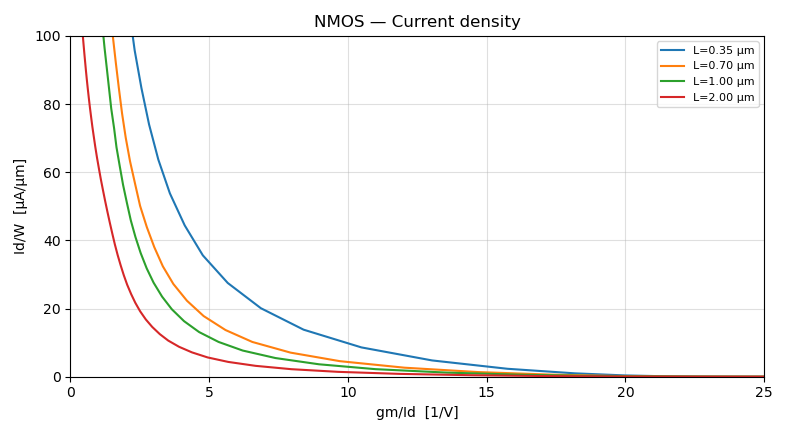
\includegraphics[width=0.9\columnwidth]{nmos_current_density.png}}
  \caption{Current density $I_D/W$ vs.\ $g_m/I_D$ for four NMOS channel
           lengths.  Read the current density at the chosen $g_m/I_D$ target,
           then apply \eqref{eq:width} to find width.}
  \label{fig:id_wl}
\end{figure}

\begin{figure}[htbp]
  \centerline{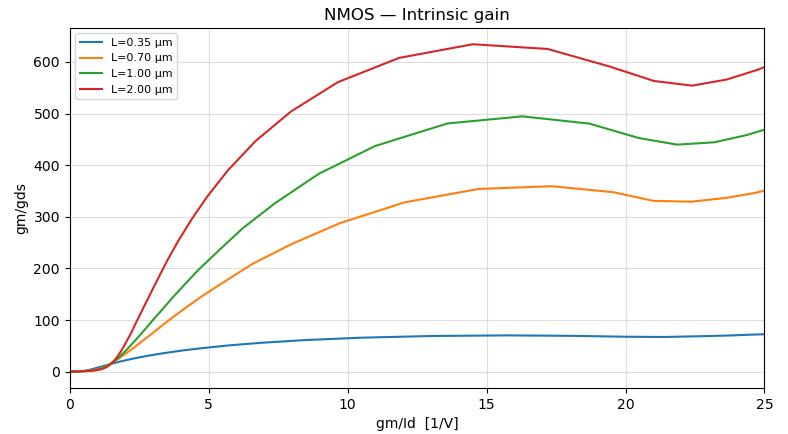
\includegraphics[width=0.9\columnwidth]{nmos_intrinsic_gain.png}}
  \caption{Intrinsic gain $g_m/g_{ds}$ vs.\ $g_m/I_D$ for four NMOS channel
           lengths.  Longer channels yield higher gain but reduce $f_T$.}
  \label{fig:gmgds}
\end{figure}

\begin{figure}[htbp]
  \centerline{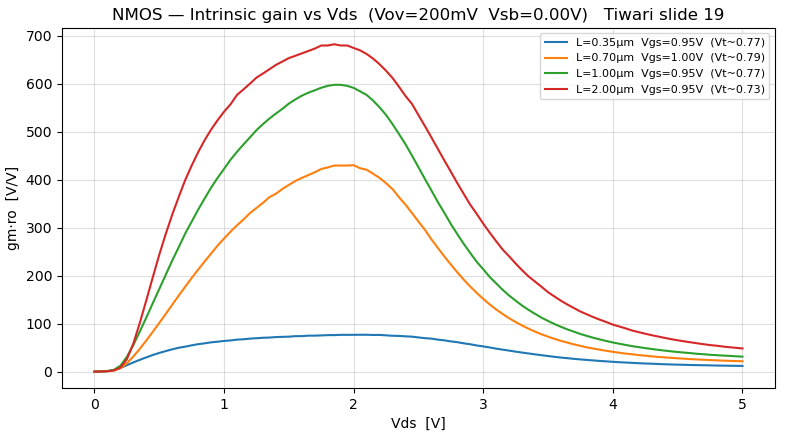
\includegraphics[width=0.9\columnwidth]{nmos_intrinsic_gain_vs_vds.png}}
  \caption{Intrinsic gain $g_m r_o$ vs.\ $V_{DS}$ at $V_{ov} = 200\,\text{mV}$,
           $V_{SB} = 0$.  Gain peaks near $V_{DS} \approx 2\,\text{V}$ and
           falls at both extremes.}
  \label{fig:gmgds_vds}
\end{figure}

\begin{figure}[htbp]
  \centerline{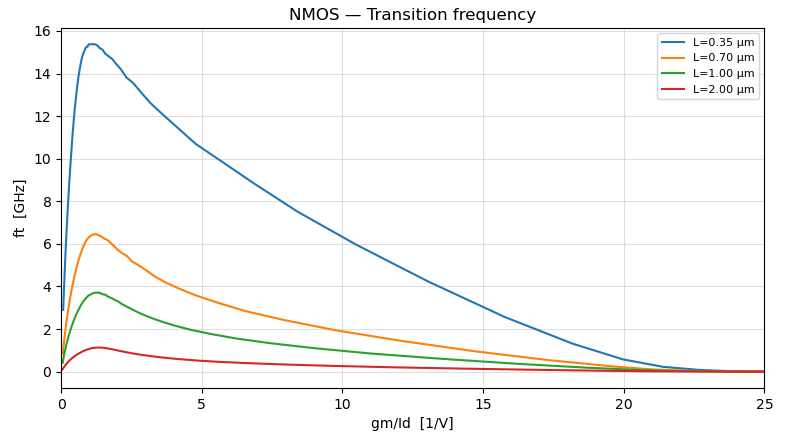
\includegraphics[width=0.9\columnwidth]{nmos_transition_frequency.png}}
  \caption{Transition frequency $f_T$ vs.\ $g_m/I_D$.  Higher $f_T$ requires
           stronger inversion (lower $g_m/I_D$) and draws more quiescent
           current.  Minimum-length devices are fastest.}
  \label{fig:ft}
\end{figure}

% ─────────────────────────────────────────────────────────────────────────────
\section{Conclusion}
\label{sec:conclusion}
% ─────────────────────────────────────────────────────────────────────────────

A Python-based gm/Id characterization and query tool has been presented.
The tool automates the characterization sweep, stores results in a
four-dimensional LUT, and provides a design-mode query that converts a
$g_m/I_D$ target and required current into a transistor width in a single
step.  The methodology was demonstrated by sizing the cascode and output-stage
transistors of a folded-cascode class-AB operational amplifier, including
an explicit inversion-level trade-off for the output devices.  Because all
sizing data come directly from the SPICE model, the results are more accurate
than square-law estimates, and minimal hand-calculation iteration is required
before running the verification simulation.

% ─────────────────────────────────────────────────────────────────────────────
\section*{Acknowledgment}
% ─────────────────────────────────────────────────────────────────────────────

The author thanks the Department of Electrical Engineering at Tarleton State
University for providing access to simulation resources in addition to Dr. Eric
Wyers for his help with this project.

\bibliographystyle{IEEEtran}
\bibliography{references}

\end{document}
